\documentclass{article}

\usepackage{neurips_2026}
\makeatletter
\renewcommand{\@noticestring}{}
\makeatother
\nolinenumbers

\usepackage[utf8]{inputenc}
\usepackage[T1]{fontenc}
\usepackage[hidelinks]{hyperref}
\usepackage{url}
\usepackage{booktabs}
\usepackage{amsfonts}
\usepackage{nicefrac}
\usepackage{microtype}
\usepackage{amsmath}
\usepackage{graphicx}
\usepackage{multirow}
\usepackage{xcolor}

\title{Does Preference Optimization Fix Chain-of-Thought Degradation?}

\author{
  Anonymous Author(s) \\
  Affiliation \\
  Address \\
  \texttt{email}
}

\begin{document}

\maketitle

\begin{abstract}
Chain-of-Thought (CoT) prompting collapses as problems grow harder, and recent work argues the traces themselves are pattern replication rather than inference. Can Direct Preference Optimization (DPO) fix the degradation---and if so, is the fix reasoning or just better pattern matching? On two open 7--8B bases (LLaMA-2-7B, Llama 3.1-8B) and two tasks (PEMDAS, CoinFlip) we evaluate five DPO interventions plus symbolic verification at inference. Multi-Domain DPO modestly raises PEMDAS accuracy on both bases, but its effect on the complexity curve splits sharply: degradation halves on LLaMA-2-7B and roughly doubles on Llama 3.1-8B. A matched diagnostic (correct vs.\ scrambled intermediates with identical final answers) exposes a base-model interaction: a 6.5 pp gap on LLaMA-2-7B but only 1.3 pp on Llama 3.1-8B, consistent with the stronger base learning format rather than reasoning. A canonical Chain-of-Preference Optimization (CPO) run with Tree-of-Thought search and model self-evaluation yields the same data-starvation regime as verifier-based Step-Level DPO: a small effect on LLaMA-2-7B and bit-identical accuracy and degradation to base on Llama 3.1-8B. Verify-and-correct on the model's own CoT recovers \emph{zero} additional accuracy on every (model, variant) combination---94--98\% of responses contain no parseable arithmetic line and the rare emitted steps are already correct; trace correctness stays below 5\% across all variants. In this 7--8B, low-data, single-run setting we do not find robust evidence that DPO (naturalistic or ToT-driven) fixes hard-instance CoT degradation; hybrid systems that pair an external symbolic backend with a generator trained to emit decomposable traces look more promising.
\end{abstract}

% ============================================================
\section{Introduction}

Chain-of-Thought (CoT) prompting is the dominant method for eliciting step-by-step reasoning from large language models~\cite{wei2022cot}, but two recent findings undermine its standing: CoT accuracy degrades sharply with problem complexity~\cite{stechly2024thoughtlessness}, and reasoning traces are unfaithful pattern replications rather than genuine inference~\cite{zhao2024mirage}. Stechly et al.\ watched GPT-4 Turbo accuracy on Last Letter Concatenation crater from ${\sim}88\%$ to under 6\% as input length grew from 1--3 to 18--20 words, with incorrect CoT traces visually indistinguishable from correct ones. Zhao et al.\ showed CoT hitting 100\% in-distribution and collapsing under distribution shift, with traces decoupled from answers.

The natural fix is preference optimization: train the model to prefer correct reasoning paths via Direct Preference Optimization (DPO)~\cite{rafailov2023dpo}, with Zhang et al.~\cite{zhang2024cpo} extending that signal to the step level via Tree-of-Thought search (CPO). We ask whether DPO fixes CoT degradation, and if so whether the fix reflects reasoning or better pattern matching, through five interventions:
\begin{enumerate}
  \item \textbf{Step-level preference pairs}: DPO at each intermediate step, not just the final answer.
  \item \textbf{Multi-domain preference data}: joint DPO on PEMDAS+CoinFlip, testing whether mixed coverage helps PEMDAS.
  \item \textbf{Diagnostic ablation (Incorrect-CoT DPO)}: pairs with correct final answers but scrambled intermediates, separating reasoning gains from pattern-matching gains.
  \item \textbf{Canonical CPO}: ToT search at training time with the model's own self-evaluation as the value function (no symbolic verifier), testing whether ToT-driven pairs surface signal that verifier-based Step-Level DPO misses.
  \item \textbf{Symbolic verification at inference}: post-hoc symbolic check on the model's own CoT, testing whether the bottleneck is learning or execution.
\end{enumerate}

% ============================================================
\section{Related Work}

\textbf{CoT prompting and its limitations.} Wei et al.~\cite{wei2022cot} introduced CoT, showing step-by-step reasoning improves LLM performance on arithmetic and symbolic tasks. Stechly et al.~\cite{stechly2024thoughtlessness} showed CoT fails to generalize beyond demonstrated step counts; Zhao et al.~\cite{zhao2024mirage} framed CoT generalization as bounded by distribution discrepancy and argued traces are pattern replications decoupled from answers.

\textbf{Preference optimization for LLMs.} Rafailov et al.~\cite{rafailov2023dpo} proposed DPO as a stable alternative to RLHF. Zhang et al.~\cite{zhang2024cpo} extended this to CoT reasoning with CPO, using ToT search to construct step-level preference pairs without ground-truth labels. Our symbolic verification experiments ask whether external verification can address the execution bottleneck that preference optimization alone cannot.

% ============================================================
\section{Method}

We use the standard DPO objective~\cite{rafailov2023dpo} with LoRA~\cite{hu2022lora} fine-tuning. Following Stechly et al., we report a \textit{degradation delta} $\Delta = \bar{a}_\mathrm{hard} - \bar{a}_\mathrm{easy}$, the gap in mean accuracy between the top and bottom thirds of complexity levels (more negative $=$ greater degradation; $\Delta \approx 0$ indicates robustness).

\subsection{Step-Level Preference Pairs}
\label{sec:method-step}

Instead of pairing entire correct vs.\ incorrect traces, we create preference pairs at each intermediate reasoning step $i$:
\begin{itemize}
  \item \textbf{Chosen}: correct step $i$ given correct prefix steps $1 \ldots i{-}1$
  \item \textbf{Rejected}: incorrect step $i$ given the same correct prefix
\end{itemize}
For PEMDAS, step correctness is \textit{symbolically verified} by evaluating intermediate arithmetic expressions with Python's \texttt{eval()}, eliminating reliance on the model's own judgment. We sample 8 traces per instance at temperature 0.8 and extract step-level pairs from instances with 4--10 operations.

\subsection{Multi-Domain DPO}

We generate correct-vs-incorrect preference pairs for both benchmark domains by sampling 6 traces per instance and combining into a single DPO run. We frame this as \emph{mixed-domain joint training} rather than cross-domain transfer, since both domains appear in both train and eval. The mix is CoinFlip-dominated on LLaMA-2-7B (711 vs.\ 143 pairs) and balanced on Llama 3.1-8B (247 vs.\ 225); §\ref{sec:pemdas-only} reports a matched PEMDAS-only ablation. LastLetterConcatenation is excluded for the same reason as in evaluation (§\ref{sec:experiments}).

\subsection{Diagnostic Ablation: Synthetic vs.\ Incorrect-CoT DPO}

Following the incorrect-CoT methodology of Stechly et al., we compare a correct-reasoning DPO variant against one whose chosen traces have scrambled intermediate steps but the same final answer. Because both bases rarely emit multi-step arithmetic under zero-shot CoT (typically one-line responses like ``The answer is 9''), model-sampled traces contain almost no intermediate content to scramble; we therefore synthesise chosen traces algorithmically to guarantee substantive steps.

\textbf{Synthetic chosen traces.} For each PEMDAS instance we parse the expression from the prompt and reduce it left-to-right using Python: innermost parentheses first, then a left-to-right pass respecting precedence. Each reduction becomes one line in the form ``$a\ \textrm{op}\ b = c$'', followed by a final ``\texttt{Answer: <value>}'' line. This yields chosen traces with a mean of 6.5 intermediate arithmetic steps ($\geq 2$ guaranteed by construction).

\textbf{Rejected traces.} Same stepwise format as chosen but with the final declared answer perturbed by a random integer offset in $\{\pm 1, \pm 2, \pm 3\}$. Both variants therefore share the same rejected distribution; the only controlled difference between the correct-CoT and incorrect-CoT variants is whether the chosen trace's intermediate steps are correct.

\textbf{Corruption procedure.} Each arithmetic line in a chosen trace receives one of three independent perturbations: \emph{swap\_operands} (skipped on commutative operators), \emph{wrong\_op} (operator that yields a value different from the declared $c$), or \emph{wrong\_result} (perturb $c$ by a random offset in $\{\pm 1, \pm 2, \pm 3\}$; disabled on the last line so the final answer is preserved). All 650 intermediate steps across the 100 synthesised traces are successfully perturbed. If DPO on corrupted pairs matches DPO on correct synthetic pairs, the improvement is consistent with pattern matching rather than with learning correct step-by-step reasoning.

\subsection{Canonical Chain-of-Preference Optimization (CPO)}
\label{sec:method-cpo}

We implement the canonical CPO setup of Zhang et al.~\cite{zhang2024cpo}: at each tree depth we sample $B{=}8$ candidate next-steps conditioned on the verified prefix, score each with the model's own self-evaluation (logit gap between `` Yes''/`` No'' on ``Is this step useful?''), append the top candidate to the chosen path, and pair every strictly lower-scoring candidate as rejected. We expand to depth 5, sampling at temperature 0.7 ($\textrm{top-}k{=}20$, $\textrm{top-}p{=}0.9$, repetition-penalty 1.15 for MPS numerical stability). To prevent self-eval errors from actively poisoning DPO, we drop pairs where the chosen step is symbolically wrong \emph{and} the rejected step is right; the symbolic check is only an anti-poisoning filter, never the value function---the search and scoring match Zhang et al.\ exactly.

\subsection{Symbolic Verification at Inference}
\label{sec:method-symbolic}

We implement two post-hoc modes over the model's own generated CoT (no replanning). \emph{Verify-only} matches each line against the arithmetic-step regex (§\ref{sec:experiments}), evaluates the LHS with Python \texttt{eval()}, and compares to the stated RHS---per-trace correctness feeds the ``Trace-correct'' and ``Has-step'' columns of Table~\ref{tab:faithfulness}. \emph{Verify-and-correct} overwrites the model's RHS with the symbolic result before re-extracting the final answer, bounding what post-hoc patching can recover \emph{given the model's own decomposition} (Table~\ref{tab:symbolic}). CoinFlip is excluded from the symbolic comparison because a structured coin-state solver trivially reaches 100\% by construction.

% ============================================================
\section{Experiments}
\label{sec:experiments}

\textbf{Models and Hardware.} LLaMA-2-7B~\cite{touvron2023llama2} (6.74B params, 2T pretraining tokens) and Llama 3.1-8B~\cite{grattafiori2024llama3} (8.03B params, 15T tokens) on Apple Silicon M5 Max (128GB). DPO is trained in fp32; evaluation generation is in fp16. Greedy decoding, max 256 new tokens, single seed (42 for the 90/10 train/eval split).

\textbf{DPO hyperparameters (all variants).} TRL DPOTrainer with $\beta{=}0.2$, learning rate $5{\times}10^{-6}$ (cosine schedule, 10\% warmup, AdamW), 3 epochs, batch size 1 $\times$ gradient accumulation 4, max sequence length 1024, no explicit reference model (TRL implicit copy of the base). LoRA: $r{=}8$, $\alpha{=}16$, dropout 0.05, attention-only target modules \{\texttt{q\_proj, k\_proj, v\_proj}\} (verified post-hoc from saved adapters; non-LLaMA names in the requested config were silently skipped by PEFT).

\textbf{Data protocol.} Preference pairs use four sampling regimes: \emph{full-trace naturalistic} (Multi-Domain, PEMDAS-only, CoinFlip-only) draws $n{=}6$ samples per instance at temperature 0.8 from each domain's full pool; \emph{Step-Level DPO} draws $n{=}8$ samples from the PEMDAS 4--10-operation subset (§\ref{sec:method-step}); \emph{synthetic} (Synthetic-CoT, Incorrect-CoT) uses $n{=}1$ deterministic synthesis restricted to instances with \texttt{steps\_to\_solve}${\le}12$ that yield ${\ge}2$ reductions, producing 100 matched pairs shared across variants; \emph{CPO} runs the ToT search of §\ref{sec:method-cpo} on PEMDAS $3{\le}\texttt{steps\_to\_solve}{\le}30$ (280 instances), with two seeds on Llama 3.1-8B to compensate for its lower yield. DPOTrainer holds 10\% of pairs as a training-time eval split (\texttt{seed=42}). Final pair counts (LLaMA-2-7B / Llama 3.1-8B): PEMDAS-only 143/225, CoinFlip-only 711/247, Multi-Domain 854/472, Step-Level 8/15, Synthetic-CoT 100/100, Incorrect-CoT 100/100, CPO 353/145. Evaluation runs on the full 290 PEMDAS / 280 CoinFlip benchmarks; because preference traces are model-generated from the same instance pool, train/eval prompts overlap by construction and we do not claim out-of-distribution generalization.

\textbf{Benchmarks.} 570 subsampled instances: PEMDAS (290, steps 2--30, 29 levels) and CoinFlip (280, 28 levels in 1--29 flips with $k{=}20$ omitted), 10 instances per level. LastLetterConcatenation is excluded because both bases fail to produce parseable zero-shot CoT responses even at 1--3 words (where GPT-4 Turbo with manual CoT reaches ${\sim}88\%$~\cite{stechly2024thoughtlessness}), making the accuracy floor uninformative.

\textbf{Metrics.}
\begin{itemize}
  \item Overall accuracy and degradation delta $\Delta$ (standard)
  \item \textbf{Trace correctness}: share of instances where (a) the response contains at least one parseable arithmetic step, (b) every parseable step is symbolically correct, and (c) the final answer is correct. Narrower than the causal-intervention faithfulness of Lanham et al.~\cite{lanham2023faithfulness}: we never intervene on the CoT and only check whether the emitted trace is arithmetically valid and consistent with the final answer. Steps are parsed with the regex \texttt{(-?\textbackslash d+\textbackslash .?\textbackslash d*)\textbackslash s*([+\textbackslash -*/])\textbackslash s*(-?\textbackslash d+\textbackslash .?\textbackslash d*)\textbackslash s*=\textbackslash s*(-?\textbackslash d+\textbackslash .?\textbackslash d*)} with LHS verified via Python \texttt{eval()}. We do not report mean step accuracy separately because the per-instance denominator is degenerate (almost all responses have 0 or 1 parseable steps).
\end{itemize}

\textbf{Experimental Conditions.}
\begin{enumerate}
  \item Base model (zero-shot CoT), for both LLaMA-2-7B and Llama 3.1-8B
  \item Multi-Domain DPO (PEMDAS + CoinFlip preference pairs; naturalistic model-sampled traces; mixed-domain joint training---see §\ref{sec:pemdas-only} for the PEMDAS-only ablation)
  \item Step-Level DPO (per-step symbolic ground-truth pairs)
  \item Synthetic-CoT DPO (synthesised multi-step PEMDAS traces with correct intermediates)
  \item Incorrect-CoT DPO (same synthesised traces with corrupted intermediates, correct final answer; diagnostic paired with 4)
  \item CPO (ToT search with model self-evaluation as value function; §\ref{sec:method-cpo})
  \item Symbolic verification: $\{$Base, DPO$\} \times \{$no verification, verify-and-correct$\}$
\end{enumerate}

% ============================================================
\section{Results}

\subsection{Main Results}
\label{sec:main-results}

Table~\ref{tab:main-results} reports zero-shot CoT accuracy and $\Delta$ for all variants on both bases, with GPT-4 Turbo from Stechly et al.~\cite{stechly2024thoughtlessness} as external reference. Multi-Domain DPO improves PEMDAS on both bases (25.5\%$\to$32.4\% on LLaMA-2-7B, 32.1\%$\to$34.8\% on Llama 3.1-8B); our best variant still sits ${\sim}21$ pp below GPT-4 Turbo, indicating substantial scale-driven headroom. CoinFlip hovers near chance across variants.

The $\Delta$ column reveals a pattern not visible from overall accuracy. Multi-Domain DPO \emph{reduces} degradation on LLaMA-2-7B ($\Delta=-13.3$ vs.\ $-27.8$) but \emph{worsens} it on Llama 3.1-8B ($-21.1$ vs.\ $-10.0$): the 2.7 pp overall gain is concentrated at easy problems, with hard-instance accuracy unchanged. DPO on naturalistic preference data therefore does not uniformly help the hard end; in one case the accuracy gain coincides with \emph{increased} complexity sensitivity.

The matched diagnostic (identical rejected distribution; chosen traces differ only in intermediate correctness) shows a base-model interaction. On LLaMA-2-7B, Synthetic-CoT beats Incorrect-CoT by \textbf{6.5 pp} (31.0\% vs.\ 24.5\%) with $\Delta$ flattening from $-30.0$ to $-14.4$---correct intermediates provide real training signal at this scale. On Llama 3.1-8B the gap collapses to \textbf{1.3 pp} (33.4\% vs.\ 32.1\%) with comparable degradation, consistent with pattern matching on the stronger base (the two models differ in family, data, and recipe, so this is not a clean test of parameter count).

\begin{table}[h]
\centering
\caption{Zero-shot CoT accuracy (\%) and degradation delta $\Delta$ (pp, hard $-$ easy; more negative $=$ greater degradation) across model variants on PEMDAS and CoinFlip. Easy/hard are the bottom/top thirds of complexity levels. The GPT-4 Turbo row is an external reference (zero-shot CoT, overall accuracy from Stechly et al.~\cite{stechly2024thoughtlessness} Table~2); per-complexity buckets are not reported there in the same form, so $\Delta$ is omitted.}
\label{tab:main-results}
\begin{tabular}{llrrrr}
\toprule
 & & \multicolumn{2}{c}{PEMDAS} & \multicolumn{2}{c}{CoinFlip} \\
\cmidrule(lr){3-4}\cmidrule(lr){5-6}
Base Model & Variant & Acc & $\Delta$ & Acc & $\Delta$ \\
\midrule
GPT-4 Turbo (ref.) & Zero-shot CoT~\cite{stechly2024thoughtlessness} & 56.1 & --- & 95.7 & --- \\
\midrule
\multirow{7}{*}{LLaMA-2-7B} & Base & 25.5 & $-27.8$ & 53.2 & $+13.3$ \\
 & Multi-Domain DPO & 32.4 & $-13.3$ & 48.9 & $-5.6$ \\
 & PEMDAS-only DPO & 33.1 & $-10.0$ & 48.6 & $-2.2$ \\
 & Step-Level DPO & 25.5 & $-27.8$ & 53.2 & $+13.3$ \\
 & Synthetic-CoT DPO & 31.0 & $-14.4$ & 53.2 & $+12.2$ \\
 & Incorrect-CoT DPO & 24.5 & $-30.0$ & 53.2 & $+13.3$ \\
 & CPO & 26.9 & $-23.3$ & 52.9 & $+12.2$ \\
\midrule
\multirow{7}{*}{Llama 3.1-8B} & Base & 32.1 & $-10.0$ & 48.2 & $+3.3$ \\
 & Multi-Domain DPO & 34.8 & $-21.1$ & 50.4 & $+5.6$ \\
 & PEMDAS-only DPO & 33.8 & $-17.8$ & 50.0 & $+4.4$ \\
 & Step-Level DPO & 31.7 & $-8.9$ & 48.6 & $+4.4$ \\
 & Synthetic-CoT DPO & 33.4 & $-13.3$ & 49.3 & $+5.6$ \\
 & Incorrect-CoT DPO & 32.1 & $-11.1$ & 47.9 & $+4.4$ \\
 & CPO & 32.1 & $-10.0$ & 49.3 & $+6.7$ \\
\bottomrule
\end{tabular}
\end{table}

Step-Level DPO yielded only 8/15 preference pairs on LLaMA-2-7B / Llama 3.1-8B (${\approx}6$--12 LoRA optimizer steps). Because LoRA $B$ is zero-initialized, the adapter begins as the identity and never escapes: trained $|B|$ is 3--4 orders of magnitude below $|A|$, and greedy outputs are byte-identical to base on LLaMA-2-7B and differ on only 18/290 PEMDAS responses on Llama 3.1-8B. Both Step-Level DPO models effectively reduce to their bases: the pair yield at this scale is below what the optimizer needs to move the adapter.

\paragraph{Ablation: PEMDAS-only naturalistic DPO.}
\label{sec:pemdas-only}
The Multi-Domain mixture is CoinFlip-dominated on LLaMA-2-7B (711 vs.\ 143 pairs) and roughly balanced on Llama 3.1-8B (247 vs.\ 225). Training the same recipe on the PEMDAS slice alone (143/225 pairs) flattens $|\Delta|$ by 3.3 pp on \emph{both} bases with overall accuracy unchanged ($\pm 1$ pp; Table~\ref{tab:main-results}). Removing CoinFlip therefore preserves the accuracy gain and worsens degradation less---suggesting the easy-skewed CoinFlip pairs drive the $\Delta$-worsening in Multi-Domain DPO rather than its PEMDAS improvement.

\subsection{Degradation Curves}

Figures~\ref{fig:pemdas-degradation-7b} and~\ref{fig:pemdas-degradation-31} plot accuracy against PEMDAS complexity $k$ for six variants per base: near 100\% at $k{=}2$, collapsing to 10--30\% by $k{\geq}10$. On LLaMA-2-7B, Multi-Domain, Synthetic-CoT, and CPO sit above base in the $k{=}10$--25 range; Incorrect-CoT tracks or drops below. On Llama 3.1-8B per-$k$ variance is larger, and CPO is visually indistinguishable from base, matching Table~\ref{tab:main-results}.

\begin{figure}[h]
\centering
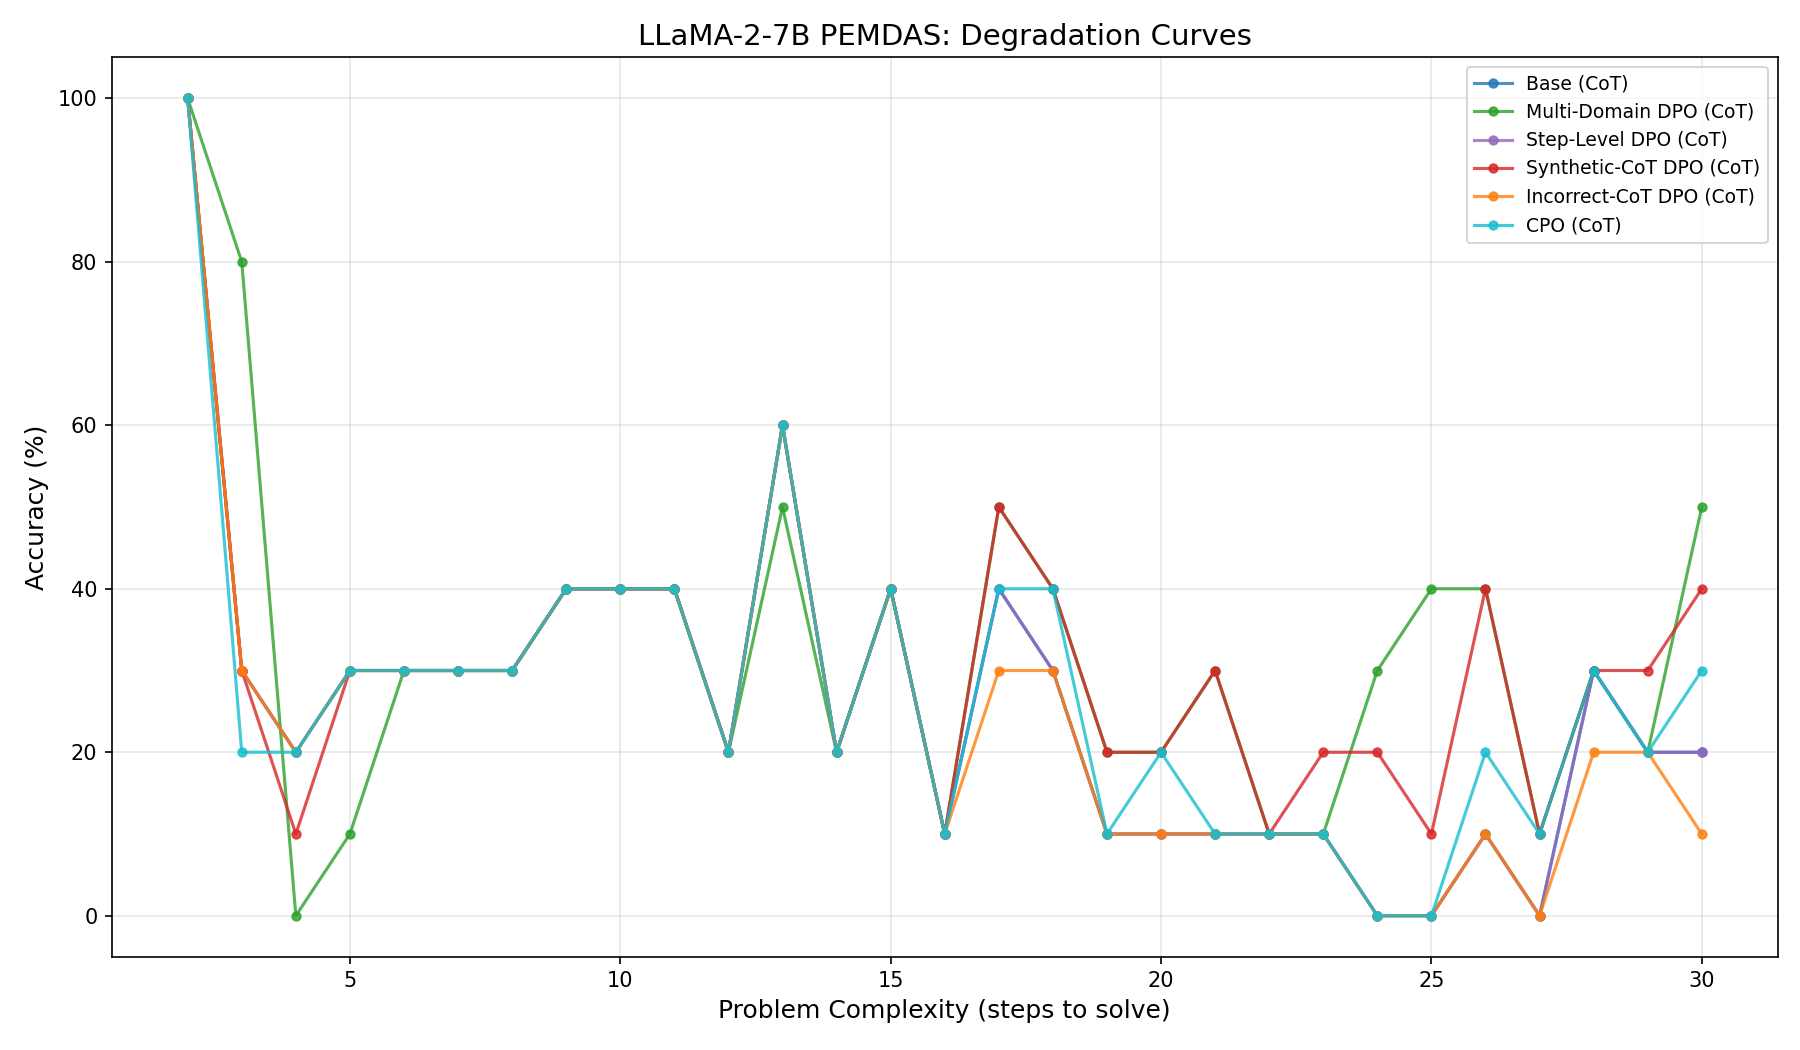
\includegraphics[width=0.85\textwidth]{figures/pemdas_all_variants.png}
\caption{LLaMA-2-7B PEMDAS: CoT accuracy vs.\ complexity. 10 instances per $k$ and a single training run per variant, so per-point variance is high; read for trend (same caveats in Figure~\ref{fig:pemdas-degradation-31}).}
\label{fig:pemdas-degradation-7b}
\end{figure}

\begin{figure}[h]
\centering
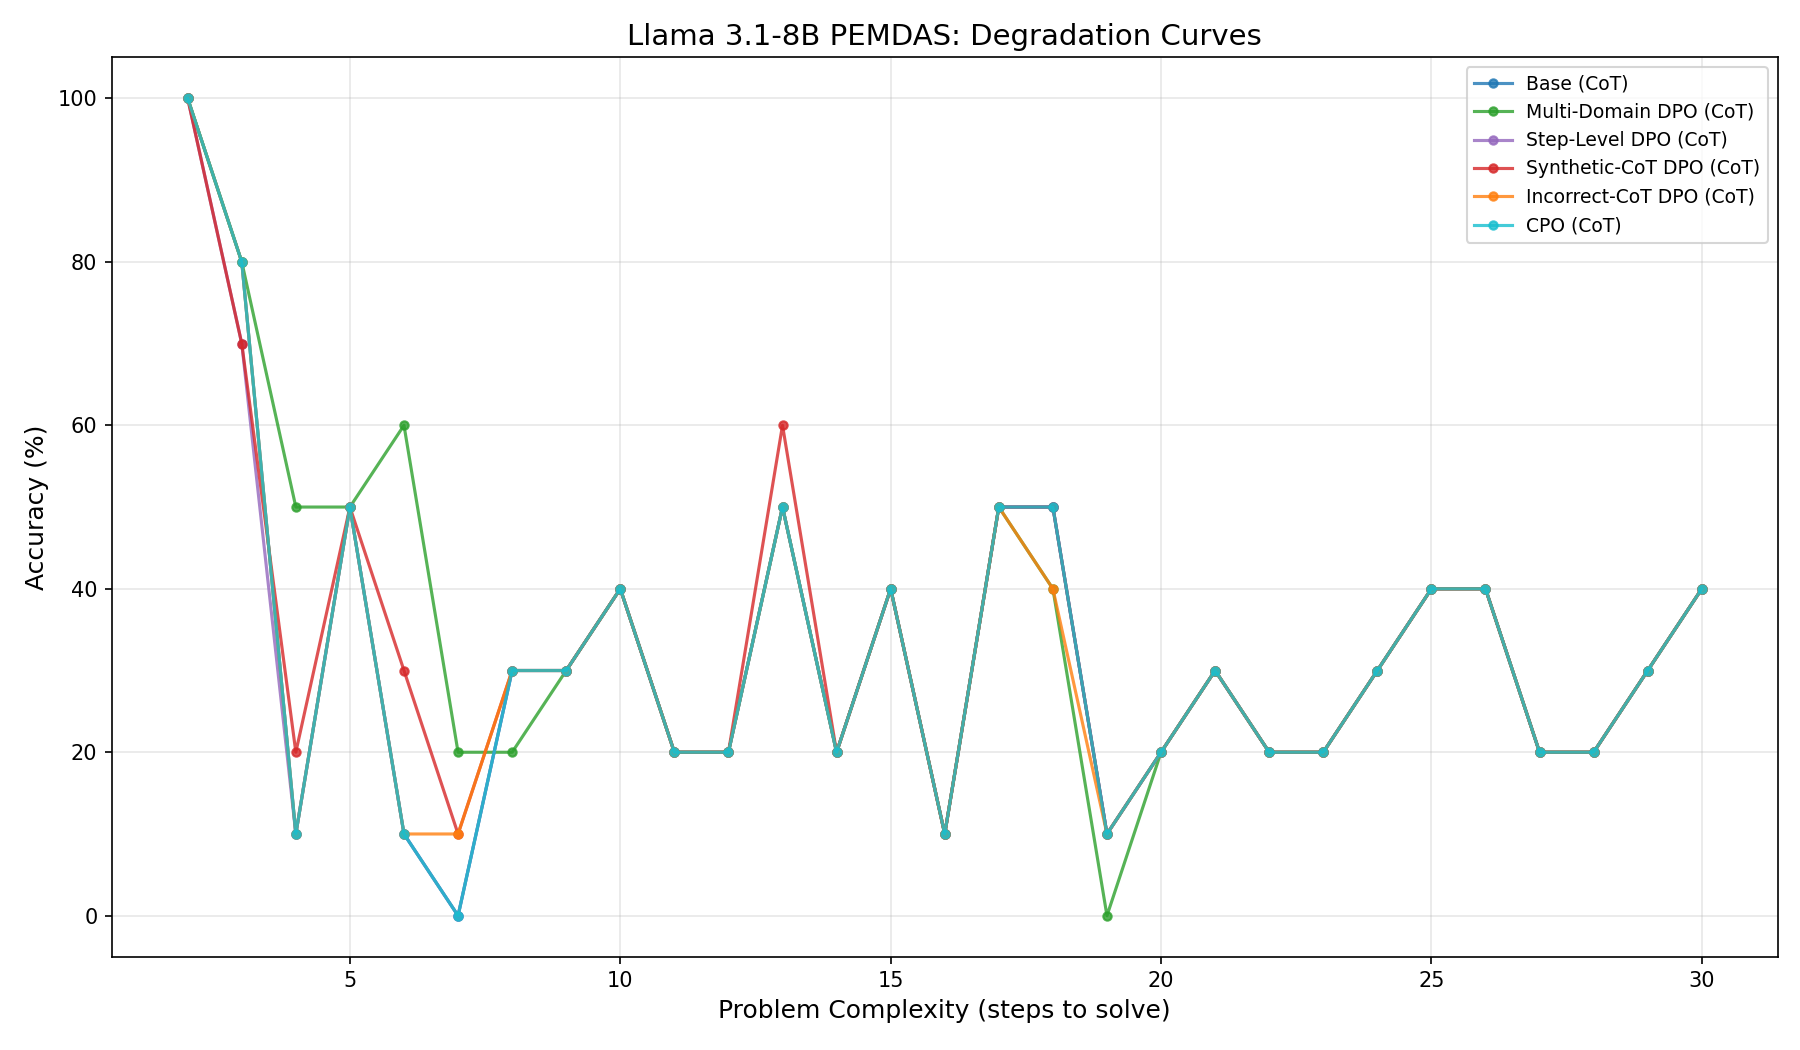
\includegraphics[width=0.85\textwidth]{figures/pemdas_llama31_variants.png}
\caption{Llama 3.1-8B PEMDAS: CoT accuracy vs.\ complexity. DPO gains concentrate at low complexity; in the Multi-Domain case the easy-only gain widens $\Delta$ despite raising mean accuracy.}
\label{fig:pemdas-degradation-31}
\end{figure}

\subsection{Trace Correctness}

Trace correctness is extremely low across all variants (Table~\ref{tab:faithfulness}). The dominant reason is not wrong intermediate steps but missing ones: 94--98\% of responses contain no parseable arithmetic line at all. Multi-Domain DPO raises the parseable-step share marginally (to 5.9\% on Llama 3.1-8B, the highest any variant reaches) but never escapes the one-line-answer regime; CPO does not change this despite being trained explicitly on per-step pairs, and trace correctness in the diagnostic variants stays at 5--7/290 on both bases. Figure~\ref{fig:faithfulness-breakdown} shows the ``wrong-trace, right answer'' bucket accounts for 22--32\% of instances, while fully trace-correct responses never exceed 5\%.

\begin{table}[h]
\centering
\caption{PEMDAS trace correctness under zero-shot CoT. ``Trace-correct'' = all parseable arithmetic steps correct \emph{and} final answer correct (narrower than the causal-intervention faithfulness of Lanham et al.~\cite{lanham2023faithfulness}; we never intervene on the CoT). ``Has-step'' = response contains at least one parseable arithmetic line. PEMDAS-only DPO omitted (Table~\ref{tab:main-results} ablation).}
\label{tab:faithfulness}
\begin{tabular}{llrr}
\toprule
Base Model & Variant & Trace-correct & Has-step \\
\midrule
\multirow{6}{*}{LLaMA-2-7B} & Base & 7/290 & 7/290 \\
 & Multi-Domain DPO & 11/290 & 11/290 \\
 & Step-Level DPO & 7/290 & 7/290 \\
 & Synthetic-CoT DPO & 7/290 & 7/290 \\
 & Incorrect-CoT DPO & 6/290 & 6/290 \\
 & CPO & 5/290 & 5/290 \\
\midrule
\multirow{6}{*}{Llama 3.1-8B} & Base & 5/290 & 6/290 \\
 & Multi-Domain DPO & 14/290 & 17/290 \\
 & Step-Level DPO & 4/290 & 5/290 \\
 & Synthetic-CoT DPO & 5/290 & 7/290 \\
 & Incorrect-CoT DPO & 6/290 & 8/290 \\
 & CPO & 5/290 & 7/290 \\
\bottomrule
\end{tabular}
\end{table}

\begin{figure}[h]
\centering
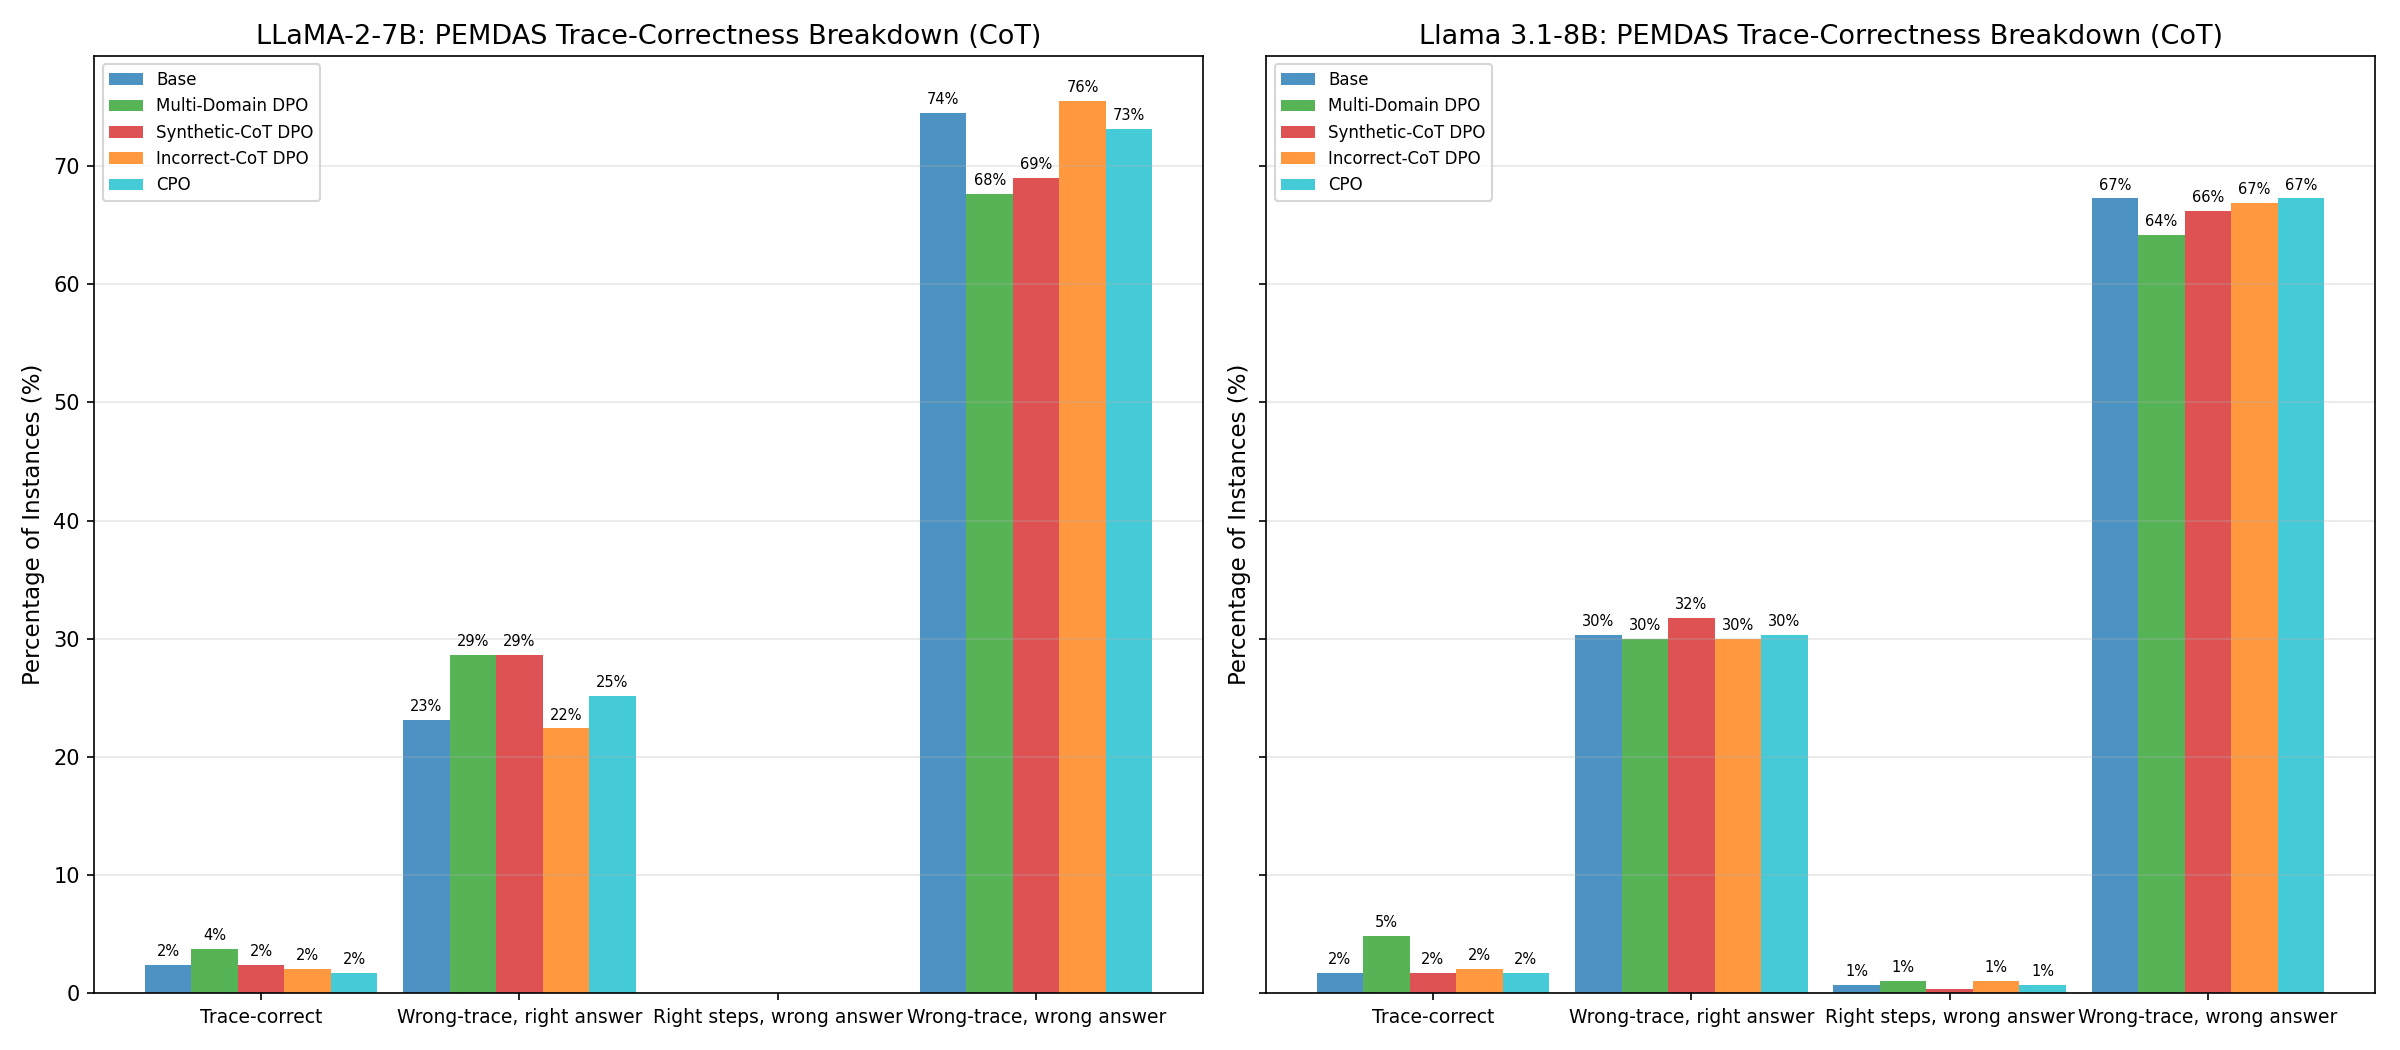
\includegraphics[width=0.85\textwidth]{figures/faithfulness_breakdown.png}
\caption{PEMDAS zero-shot CoT response breakdown. The ``wrong-trace, right answer'' bucket is dominated by responses with no parseable intermediate steps, not by explicitly wrong steps. DPO accuracy gains do not translate into trace-correct reasoning. PEMDAS-only DPO omitted (Table~\ref{tab:main-results} ablation).}
\label{fig:faithfulness-breakdown}
\end{figure}

\subsection{Symbolic Verification}
\label{sec:results-symbolic}

A deterministic Python \texttt{eval()} solver on the raw expression reaches 100\% on every variant by construction (omitted from Table~\ref{tab:symbolic}; it confirms only that the problems are solvable). The ``+ V\&C'' column overwrites each parseable step in the model's CoT with its symbolic result before re-extracting the final answer. \emph{Verify-and-correct recovers zero additional accuracy on every (model, variant) combination}: only 2--6\% of responses contain any parseable step, and where they do, the single emitted step is already correct. The gap to the oracle is entirely the ``no parseable decomposition'' regime---a generation bottleneck, not an execution one.

\begin{table}[h]
\centering
\caption{Symbolic baselines on PEMDAS (\%). ``Has-step'' is the share of 290 responses containing at least one parseable arithmetic line. ``+ V\&C'' overwrites each such RHS with the symbolic result before re-extracting the final answer; the 100\%-by-construction raw-expression oracle is omitted. PEMDAS-only DPO is a Table~\ref{tab:main-results} ablation, omitted here.}
\label{tab:symbolic}
\begin{tabular}{llrrr}
\toprule
Base Model & Variant & CoT Acc & Has-step & + V\&C \\
\midrule
\multirow{6}{*}{LLaMA-2-7B} & Base & 25.5 & 2.4 & 25.5 \\
 & Multi-Domain DPO & 32.4 & 3.8 & 32.4 \\
 & Step-Level DPO & 25.5 & 2.4 & 25.5 \\
 & Synthetic-CoT DPO & 31.0 & 2.4 & 31.0 \\
 & Incorrect-CoT DPO & 24.5 & 2.1 & 24.5 \\
 & CPO & 26.9 & 1.7 & 26.9 \\
\midrule
\multirow{6}{*}{Llama 3.1-8B} & Base & 32.1 & 2.1 & 32.1 \\
 & Multi-Domain DPO & 34.8 & 5.9 & 34.8 \\
 & Step-Level DPO & 31.7 & 1.7 & 31.7 \\
 & Synthetic-CoT DPO & 33.4 & 2.4 & 33.4 \\
 & Incorrect-CoT DPO & 32.1 & 2.8 & 32.1 \\
 & CPO & 32.1 & 2.4 & 32.1 \\
\bottomrule
\end{tabular}
\end{table}

% ============================================================
\section{Discussion}

\textbf{Pattern matching vs.\ reasoning.} The diagnostic gap shrinks from 6.5 pp on LLaMA-2-7B to 1.3 pp on Llama 3.1-8B, and the complexity-curve effect of Multi-Domain DPO flips sign between the two bases despite a similar overall accuracy gain. The simplest reading is a base-model interaction: the stronger base extracts enough format signal from any DPO run that correct-vs-scrambled intermediates barely matter, while the weaker base still responds to correct intermediates. The PEMDAS-only ablation further suggests the $\Delta$-worsening in Multi-Domain DPO comes from the easy-skewed CoinFlip pairs rather than the PEMDAS preference signal, though the control shifts both mixture and pair count (854/472 vs.\ 143/225) so the isolation is not clean.

\textbf{The bottleneck is generation, not execution.} A deterministic solver on the raw expression is perfect by construction, yet verify-and-correct over the model's own CoT recovers zero accuracy on every variant: the model rarely emits a parseable step, and where it does, the step is already correct. DPO does not escape this regime---even our best variant raises the parseable-step share only to 5.9\%. A practical hybrid system would need both an external symbolic backend and a generator trained to emit step-by-step traces; neither DPO on naturalistic CoT, nor ToT-search-driven self-eval pairs, supplies both.

\textbf{Step-level signal is data starved, even with ToT search.} Verifier-based Step-Level DPO yields 8--15 pairs and leaves adapters near identity; canonical CPO with self-evaluation (§\ref{sec:method-cpo}) yields 353/145 pairs and produces only the small LLaMA-2-7B movement, with bit-identical accuracy and degradation on Llama 3.1-8B. The bottleneck is therefore how many parseable step candidates the base can generate for the search, not which scoring function ranks them. Two factors compound this: only 47\% of 8B chosen steps are symbolically correct (vs.\ 56\% for 7B), so the self-eval value function is itself noisy at this scale; and the train/inference prefix mismatch from §\ref{sec:method-step} persists under CPO. Our results do not bound what CPO can do on a stronger or instruction-tuned base.

\textbf{Limitations.} We evaluate two 7--8B bases with a single training run per variant; larger or instruction-tuned models may behave differently. CoinFlip accuracy hovers within sampling noise of chance, so we treat its $\Delta$ as noise. Step-level analysis is restricted to PEMDAS, where step boundaries are unambiguous, and the diagnostic rests on synthetic chosen traces rather than naturalistic CoT.

% ============================================================
\section{Conclusion}

Across five DPO interventions on two 7--8B bases and two tasks, none closes the complexity gap in this setting. Multi-Domain DPO halves $\Delta$ on LLaMA-2-7B but roughly doubles it on Llama 3.1-8B; the matched diagnostic shows a base-model interaction (6.5 vs.\ 1.3 pp), consistent with pattern matching on the stronger base; and canonical CPO with ToT search yields only a small movement on 7B and bit-identical numbers to base on 8B, confirming that the step-level bottleneck is the base's ability to produce parseable decomposition candidates, not the choice of scoring function. Trace correctness stays below 5\% and 94--98\% of outputs contain no parseable decomposition---so even a perfect post-hoc verifier cannot help until the model emits one. We are not claiming preference optimization \emph{cannot} bridge the gap; we are showing that none of the five interventions tested closes it at this scale in this low-data, single-run setting. The more promising path looks hybrid: an external symbolic backend paired with a generator trained to emit decomposable traces. Code, preference data, and per-instance raw results will be released upon acceptance.

% ============================================================
\bibliographystyle{plain}

\small
\begin{thebibliography}{9}

\bibitem{wei2022cot}
J.~Wei, et~al.
\newblock Chain-of-thought prompting elicits reasoning in large language models.
\newblock In \emph{NeurIPS}, vol.~35, 2022.

\bibitem{stechly2024thoughtlessness}
K.~Stechly, K.~Valmeekam, and S.~Kambhampati.
\newblock Chain of thoughtlessness? {An} analysis of {CoT} in planning.
\newblock In \emph{NeurIPS}, vol.~37, pp.~29106--29141, 2024.

\bibitem{zhao2024mirage}
C.~Zhao, et~al.
\newblock Is chain-of-thought reasoning of {LLMs} a mirage? {A} data distribution lens.
\newblock \emph{arXiv:2508.01191}, 2025.

\bibitem{zhang2024cpo}
Z.~Zhang, et~al.
\newblock Chain of preference optimization: Improving chain-of-thought reasoning in {LLMs}.
\newblock In \emph{NeurIPS}, vol.~37, 2024.

\bibitem{rafailov2023dpo}
R.~Rafailov, et~al.
\newblock Direct preference optimization: Your language model is secretly a reward model.
\newblock In \emph{NeurIPS}, vol.~36, 2023.

\bibitem{touvron2023llama2}
H.~Touvron, et~al.
\newblock {LLaMA} 2: Open foundation and fine-tuned chat models.
\newblock \emph{arXiv:2307.09288}, 2023.

\bibitem{hu2022lora}
E.~Hu, et~al.
\newblock {LoRA}: Low-rank adaptation of large language models.
\newblock In \emph{ICLR}, 2022.

\bibitem{grattafiori2024llama3}
A.~Grattafiori, et~al.
\newblock The {L}lama 3 herd of models.
\newblock \emph{arXiv:2407.21783}, 2024.

\bibitem{lanham2023faithfulness}
T.~Lanham, et~al.
\newblock Measuring faithfulness in chain-of-thought reasoning.
\newblock \emph{arXiv:2307.13702}, 2023.

\end{thebibliography}

\end{document}
